% --------------------------------------------------
%  TALLER DE INTRODUCCIÓN A LaTeX
%  https://github.com/mianfg/latex-intro
%
%  Sesión 1 -> Presentación
%
%  Autor: Miguel Ángel Fernández Gutiérrez, @mianfg
%  Fecha: 20 febrero, 2019
% --------------------------------------------------

% Tipo de documento (presentación)
\documentclass[10pt, xcolor=table]{beamer}

% Cargar el tema
\usetheme{metropolis}

%  __________
% |          |
% | Paquetes |
% |__________|

% Paquetes de idioma
\usepackage[utf8]{inputenc}
\usepackage[spanish, es-tabla, es-lcroman, es-noquoting]{babel}

% Paquete para código fuente
% LISTINGS
\usepackage{listings}
\usepackage{lipsum}
\usepackage{courier}

% Colores para los bloques de código
\definecolor{codegreen}{rgb}{0,0.6,0}
\definecolor{codegray}{rgb}{0.5,0.5,0.5}
\definecolor{codepurple}{rgb}{0.58,0,0.82}
\definecolor{backcolour}{rgb}{0.95,0.95,0.92}
\lstdefinestyle{mystyle}{
	backgroundcolor=\color{backcolour},   
	commentstyle=\color{codegreen},
	keywordstyle=\color{blue},
	numberstyle=\tiny\color{codegray},
	stringstyle=\color{codepurple},
	basicstyle=\footnotesize\ttfamily,
	breakatwhitespace=false,         
	breaklines=true,                 
	captionpos=b,                    
	keepspaces=true,                 
	numbers=left,                    
	numbersep=5pt,                  
	showspaces=false,                
	showstringspaces=false,
	showtabs=false,                  
	tabsize=4
}
\lstset{style=mystyle}

% Paquete de numeración en Beamer
\usepackage{appendixnumberbeamer}

% Paquete de uso para plantilla
\usepackage{booktabs}
\usepackage[scale=2]{ccicons}

% Paquete para controlar espacios
\usepackage{xspace}
\newcommand{\themename}{\textbf{\textsc{metropolis}}\xspace}

% Paquetes para matemáticas
\usepackage{amsmath}    % Paquete básico de matemáticas
\usepackage{amsthm}     % Teoremas
\usepackage{mathrsfs}   % Fuente para ciertas letras utilizadas en matemáticas

% Paquetes para fuentes
\usepackage{newpxtext, newpxmath}   % Fuente similar a Palatino
\usepackage{FiraSans}               % Fuente sans serif
\usepackage[T1]{fontenc}
\usepackage[italic]{mathastext}     % Utiliza la fuente del documento
                                    % en los entornos matemáticos

%  ________________________
% |                        |
% | Configuración del tema |
% |________________________|

% Configuración básica del tema
\metroset{
  % tema oscuro ('dark') o claro ('light'). No tiene efecto al usar la
  % paleta de colores más adelante
  background=light,
  % 'none' para eliminar la diapositiva inicial de cada sección
  sectionpage=progressbar,
  % 'progressbar' o 'simple' para añadir una diapositiva inicial a cada subsección
  subsectionpage=none,
  % contador de página: 'none', 'counter' o 'fraction'
  numbering=none,
  % barra de progreso: 'none', 'head', 'frametitle' o 'foot'
  progressbar=frametitle,
  % fondo de los bloques estilo teorema: 'transparent' o 'fill'
  block=fill,
}










\usepackage[normalem]{ulem}
\usepackage{cancel}
\newcommand\dout{\bgroup \markoverwith{\rule[0.2ex]{0.1pt}{0.4pt}\rule[0.8ex]{0.1pt}{0.4pt}}\ULon}
\def\dout{\bgroup
 \markoverwith{\lower-0.35ex\hbox
 {\kern-.03em\vbox{\hrule width.2em\kern0.45ex\hrule}\kern-.03em}}%
 \ULon}
\MakeRobust\dout






% Paleta de colores
\definecolor{accent}{HTML}{4caf50}
\colorlet{darkaccent}{accent!70!black}
\definecolor{foreground}{RGB}{0, 0, 0}
\definecolor{background}{RGB}{255, 255, 255}

% Insertar los colores en el tema
\setbeamercolor{normal text}{fg=foreground, bg=background}
\setbeamercolor{alerted text}{fg=darkaccent, bg=background}
\setbeamercolor{example text}{fg=foreground, bg=background}
\setbeamercolor{frametitle}{fg=background, bg=accent}

\setbeamercolor{headtitle}{fg=background!70!accent,bg=accent!90!foreground}
\setbeamercolor{headnav}{fg=background,bg=accent!90!foreground}
\setbeamercolor{section in head/foot}{fg=background,bg=accent}

\defbeamertemplate*{headline}{miniframes theme no subsection}{
  % Caja para mostrar título y autor encima de cada diapositiva
  % Nosotros no 
  %% \begin{beamercolorbox}[ht=2.5ex,dp=1.125ex,
  %%     leftskip=.3cm,rightskip=.3cm plus1fil]{headtitle}
  %%   {\usebeamerfont{title in head/foot}\insertshorttitle}
  %%   \hfill
  %%   \leavevmode{\usebeamerfont{author in head/foot}\insertshortauthor}
  %% \end{beamercolorbox}
  %% \begin{beamercolorbox}[colsep=1.5pt]{upper separation line head}
  %% \end{beamercolorbox}

  % Caja para mostrar navegación encima de cada diapositiva
  \begin{beamercolorbox}{headnav}
    \vskip2pt\insertnavigation{\paperwidth}\vskip2pt
  \end{beamercolorbox}
  \begin{beamercolorbox}[colsep=1.5pt]{lower separation line head}
  \end{beamercolorbox}
}

%  _________
% |         |
% | Ajustes |
% |_________|

% Fijar tabla a posición
\usepackage{array}
\newcolumntype{L}[1]{>{\raggedright\let\newline\\\arraybackslash\hspace{0pt}}m{#1}}
\newcolumntype{C}[1]{>{\centering\let\newline\\\arraybackslash\hspace{0pt}}m{#1}}
\newcolumntype{R}[1]{>{\raggedleft\let\newline\\\arraybackslash\hspace{0pt}}m{#1}}

%  ________
% |        |
% | Título |
% |________|

\title{Creando una criptomoneda}
\subtitle{Fundamentos de Redes. \alert{Seminarios}}
\date{}
\author{Miguel Ángel Fernández Gutiérrez\\Pedro Gallego López\\[4pt]\footnotesize{Doble Grado en Ingeniería Informática y Matemáticas}}
\titlegraphic{\hfill
\includegraphics[width=2.5cm]{ugrlogo-dark.pdf}}

%  ___________
% |           |
% | Documento |
% |___________|

\begin{document}

\maketitle

\begin{frame}{Índice}
	\setbeamertemplate{section in toc}[sections numbered]
	\tableofcontents[]
\end{frame}

\section{¿Qué es una criptomoneda?}

\begin{frame}[fragile]{¿Qué queremos?}
\begin{center}
	
\includegraphics[width=0.8\textwidth]{./resources/logo.png}
\end{center}

\end{frame}

\begin{frame}{¿Qué queremos?}
Queremos crear un sistema \textbf{anónimo}, \textbf{descentralizado} y \textbf{seguro}.
\begin{itemize}
	\item \textbf{Anónimo:} usuarios identificables, pero no su verdadera identidad.
	\item \textbf{Descentralizado:} eliminar instituciones centrales.
	\item \textbf{Seguro:} no permitiremos transacciones fraudulentas.
\end{itemize}
\end{frame}

\begin{frame}{¿Qué queremos?}
Para que nuestro sistema tenga todo esto, deberá cumplir una serie de \textbf{requisitos}:

\hfill\begin{minipage}{1\textwidth}
\begin{enumerate}
\def\labelenumi{\emph{Req. \arabic{enumi}.}}
\itemsep1pt\parskip0pt\parsep0pt
\item[\emph{Req. 1.}]
  El sistema no requiere de una \textbf{autoridad central}: su estado es
  mantenido mediante un \textbf{consenso} distribuido.
\item[\emph{Req. 2.}]
  El sistema mantiene un \textbf{seguimiento} de todas las unidades de
  la criptomoneda y de sus propietarios.
\item[\emph{Req. 3.}]
  El sistema define si se pueden crear \textbf{nuevas unidades} de la
  criptomoneda. Si esto es así, el sistema debe definir las
  circunstancias de su origen y cómo determinar quién será el
  propietario de éstas.
\item[\emph{Req. 4.}]
  La propiedad de las monedas puede probarse de forma exclusivamente
  \textbf{criptográfica}.
\item[\emph{Req. 5.}]
  El sistema permite la realización de \textbf{transacciones} de forma
  controlada.
\end{enumerate}
\end{minipage}
\end{frame}

\begin{frame}{¿Qué queremos?}
Nuestro sistema girará en torno a las siguientes \textbf{ideas clave}:
\begin{enumerate}
\item Descentralización
\item Firmas digitales
\item La contabilidad (\emph{ledger}) es la propia moneda
\item Mecanismo de consenso
\item Blockchain
\end{enumerate}
\end{frame}

\begin{frame}{1. Descentralización: redes P2P}

\begin{itemize}
	\item Solución para descentralización: \textbf{redes P2P}.
	\item Todos los ordenadores tienen el mismo peso, información compartida de igual a igual, al contrario que cliente-servidor.
\end{itemize}

\end{frame}

\begin{frame}{1. Descentralización: redes P2P. \normalfont{Características}}

\begin{itemize}
	\item Cada nodo actúa simultáneamente como cliente y como servidor.
	\item Permiten intercambio directo de información, en cualquier formato, entre los ordenadores interconectados.
\end{itemize}

\end{frame}

\begin{frame}{1. Descentralización: redes P2P. \normalfont{Características}}
Rasgos a destacar:

\begin{itemize}
	\item \textbf{Escalabilidad:} mientras más nodos estén conectados, mejor será el funcionamiento.
	\item \textbf{Descentralización:} ningún nodo es imprescindible para el funcionamiento de la red.
	\item \textbf{Distribución de costes entre los usuarios.}
	\item \textbf{Robustez:} menos puntos singulares de fallas en el sistema.
	\item \textbf{Anonimato.}
	\item \textbf{Seguridad:} investigar nodos maliciosos. Característica deseable, poco implementada. Algunas soluciones prometedoras: \emph{cifrado multiclave, cajas de arena...}
\end{itemize}

\end{frame}

\begin{frame}{1. Descentralización: redes P2P. \normalfont{Topologías}}
\hspace{0cm}
\begin{table}[h]
\begin{tabular}{ccc}
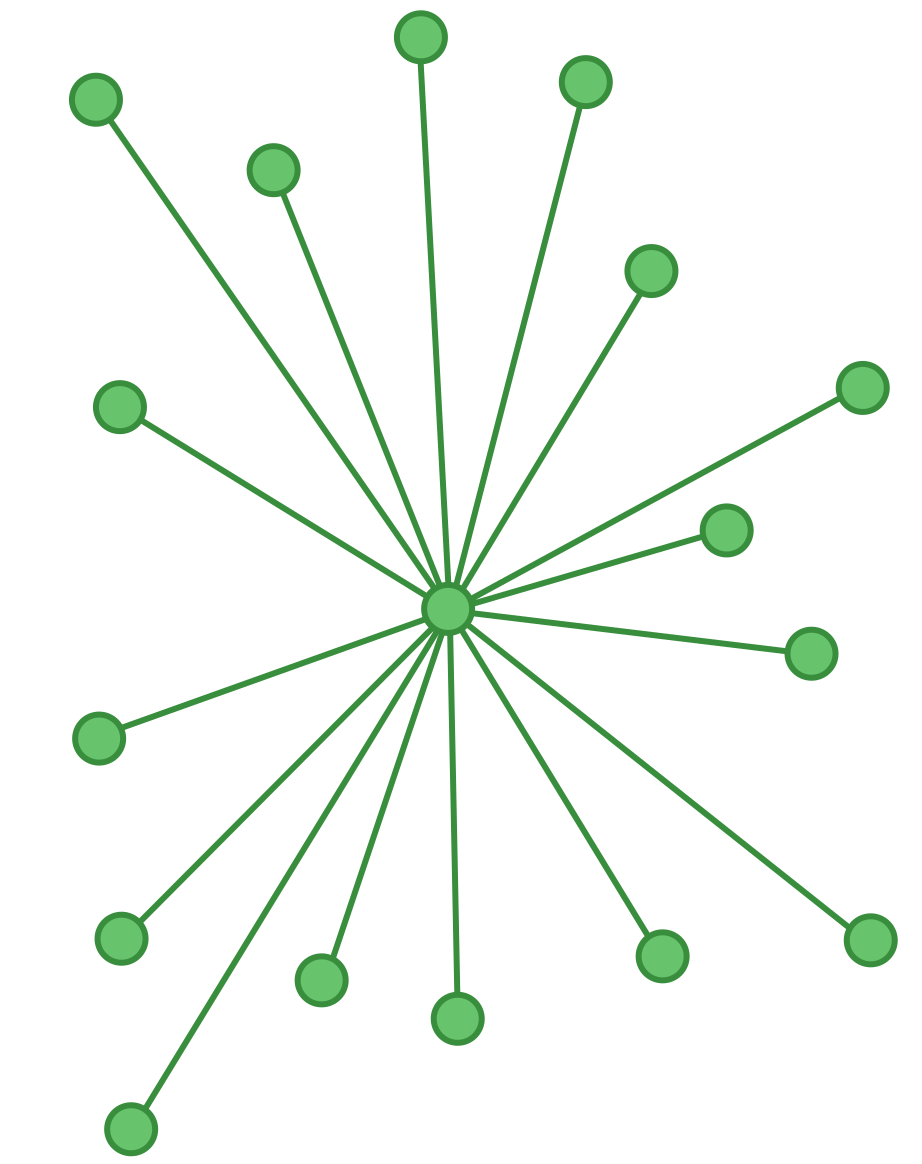
\includegraphics[width=3cm]{./resources/p2p1.png} & 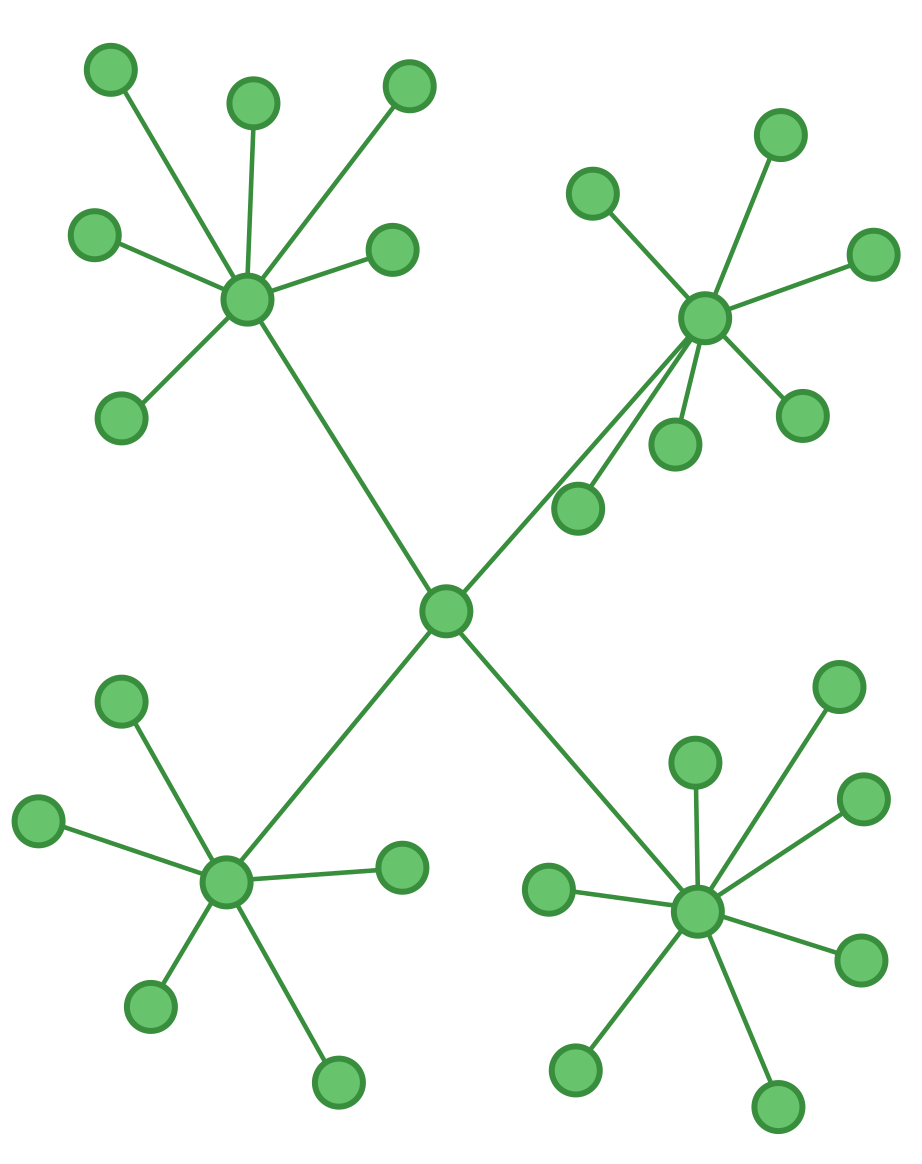
\includegraphics[width=3cm]{./resources/p2p2.png} & 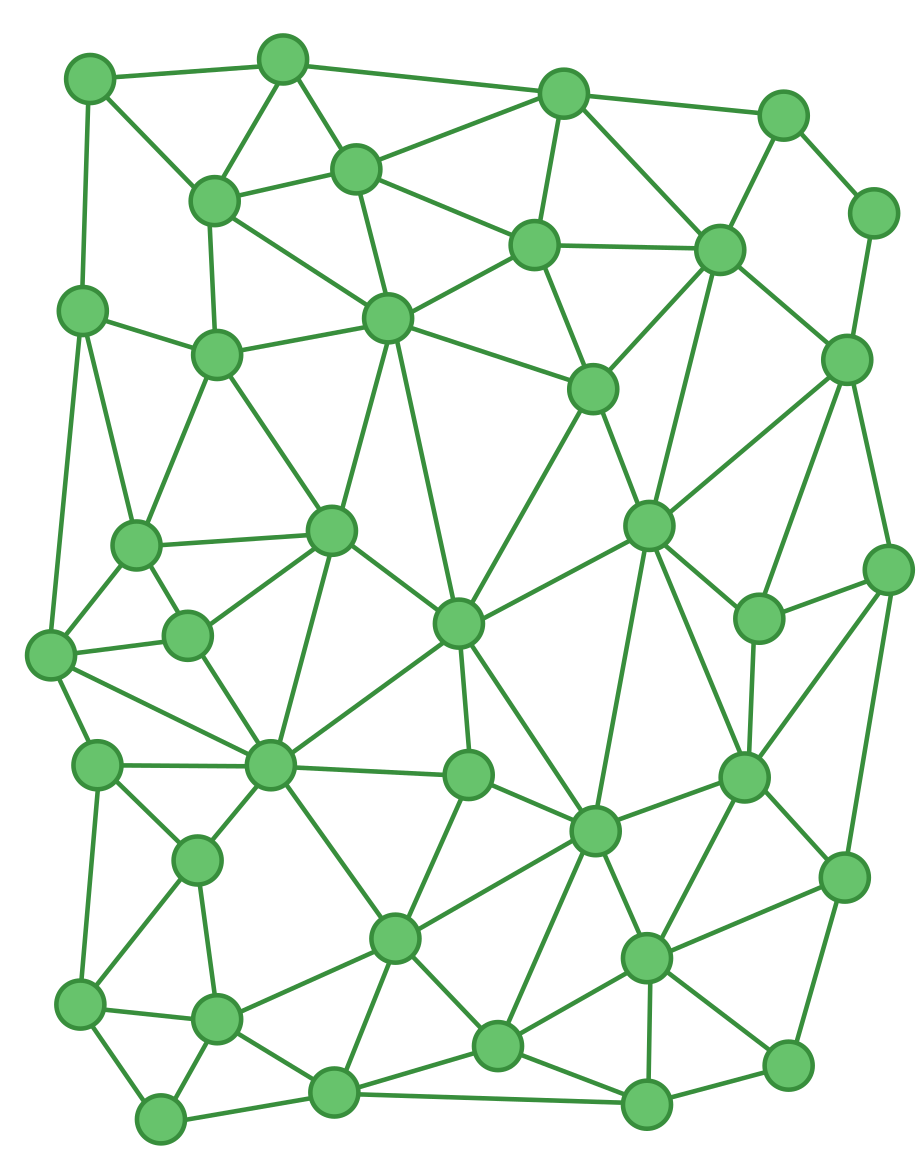
\includegraphics[width=3cm]{./resources/p2p3.png} \\
\\
centralizada & descentralizada & descentralizada\\
&y estructurada & y no estructurada\\
\end{tabular}
\end{table}

\end{frame}

\begin{frame}{1. Descentralización: redes P2P. \normalfont{Ventajas e inconvenientes}}
\large{\textbf{Ventajas}}\normalsize
\begin{itemize}
	\item \textbf{Costo:} muchos de los programas P2P son gratuitos.
	\item \textbf{Eficiencia:} compartir archivos en P2P es fácil y rápido.
\end{itemize}
\vspace{0.5cm}
\large{\textbf{Inconvenientes}}\normalsize
\begin{itemize}
	\item \textbf{Legalidad:} compartir archivos ilegales en estas redes.
\end{itemize}
\end{frame}


\begin{frame}{2. Firmas digitales, criptografía y hashing}
Para que nuestro sistema funcione son esenciales las \textbf{identidades
digitales}, es decir, formas de verificar que una transacción se ha
hecho realmente (alguien de verdad ha enviado dinero a otra persona).
Para eso, usamos la \textbf{criptografía}.
\end{frame}

\begin{frame}{2. Firmas digitales, criptografía y hashing. \normalfont{Funciones hash}}
\begin{center}
	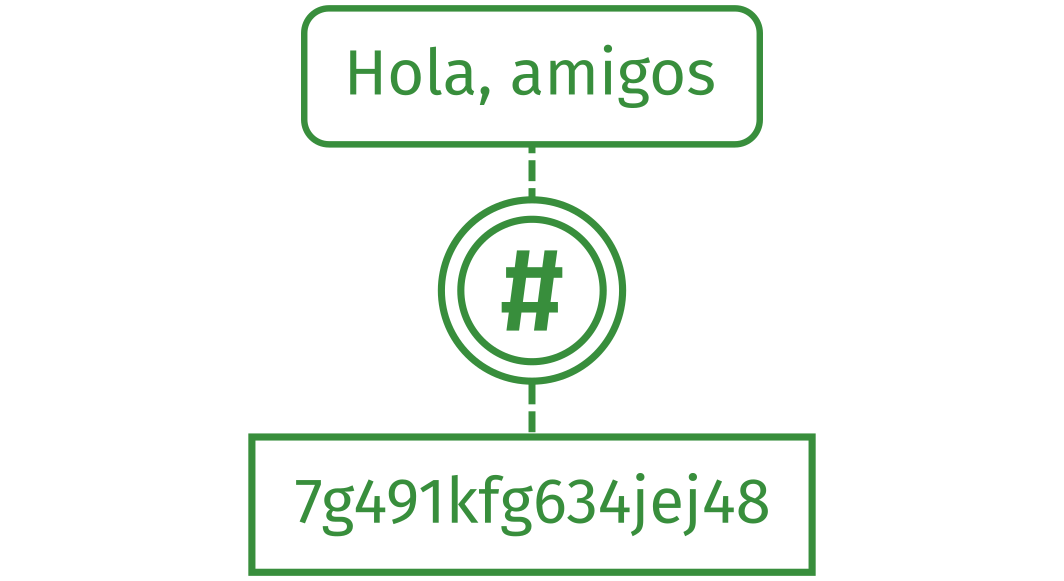
\includegraphics[width=0.8\textwidth]{./resources/hash.png}
\end{center}
\end{frame}


\begin{frame}{2. Firmas digitales, criptografía y hashing. \normalfont{Funciones hash}}
Una buena función hash debe garantizar:

\begin{enumerate}
\item
	La salida de la función hash debe tener un tamaño fijo.
\item
	Un mínimo cambio en la entrada debe producir un enorme cambio en la salida.
\item
	Una misma entrada siempre producirá la misma salida.
\item
	No debe haber forma alguna de revertir el cambio, es decir, de que a partir de la salida se pueda encontrar la entrada.
\item
	Calcular el valor hash debe ser rápido; no debe requerir de un gran trabajo computacional.
\end{enumerate}
\end{frame}


\begin{frame}{2. Firmas digitales, criptografía y hashing. \normalfont{Firmas digitales}}
Las funciones hash las usan algoritmos criptográficos, que utilizaremos para garantizar que nadie diga nada en tu nombre: \textbf{firmas digitales}.

Usaremos el método de \textbf{criptografía asimétrica} (clave privada-clave pública).
\end{frame}


\begin{frame}{2. Firmas digitales, criptografía y hashing. \normalfont{Firmas digitales}}
\begin{center}
	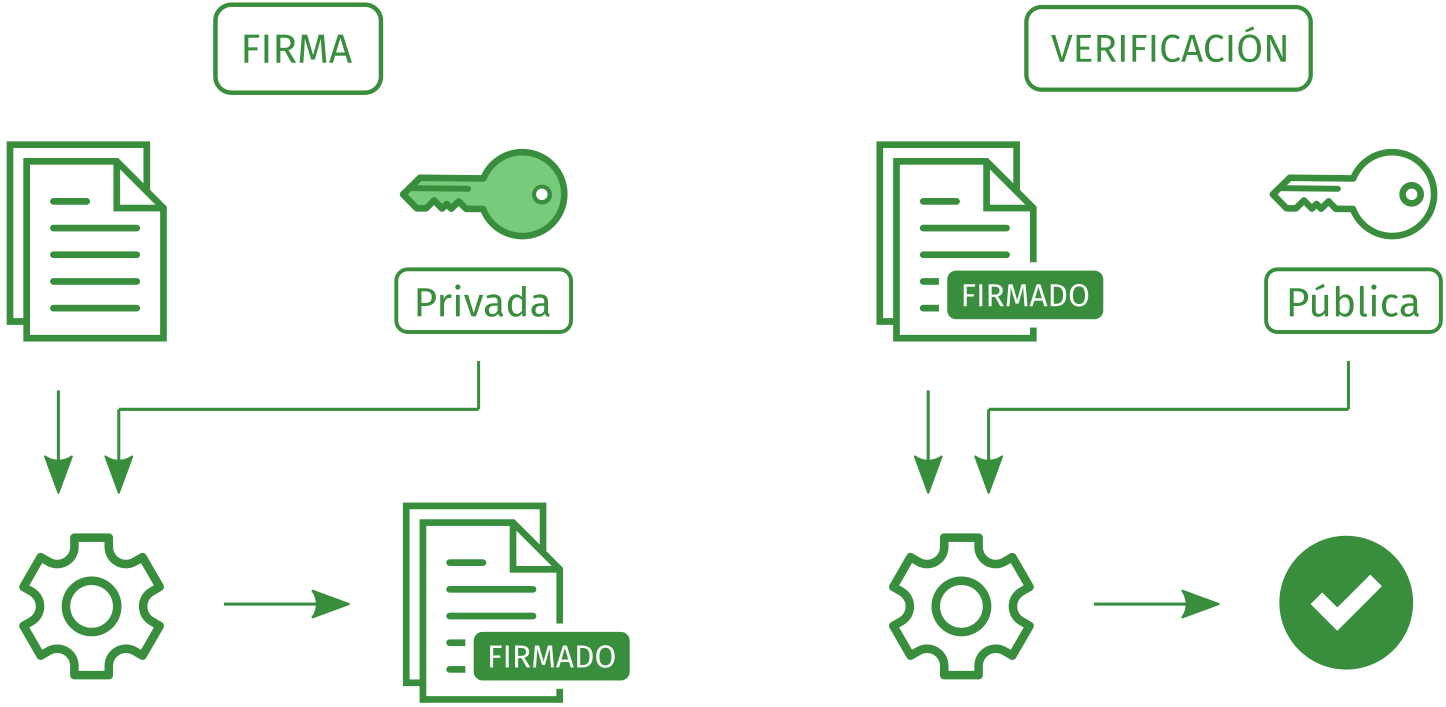
\includegraphics[width=0.9\textwidth]{./resources/signing.png}
\end{center}
\end{frame}

\begin{frame}{2. Firmas digitales, criptografía y hashing. \normalfont{Firmas digitales}}
\begin{center}
	\large Firma
\end{center}
$$
Firmar(\textbf{Mensaje}, \textbf{Clave Privada}) = \textbf{Firma}
$$
\end{frame}

\begin{frame}{2. Firmas digitales, criptografía y hashing. \normalfont{Firmas digitales}}
\begin{center}
	\large Verificación
\end{center}
$$
Verificar(\textbf{Mensaje}, \textbf{Firma}, \textbf{Clave Pública}) = \begin{cases} true \\ false \end{cases}
$$
\end{frame}


\begin{frame}{3. Enviando transacciones a la red}
\begin{itemize}
	\item Nos queda enviar información al sistema.
	\item No tenemos autoridad central que valide cuánto dinero tenemos, pero no hace falta: \textbf{la contabilidad es la propia moneda} (nos basta tener una lista de transacciones, \emph{ledger}).
\end{itemize}
\end{frame}

\begin{frame}{3. Enviando transacciones a la red}
\textbf{Ejemplo.} Listado de transacciones de un usuario en \emph{DGIIMCoin}.
\begin{enumerate}
	\item Tengo 500\dout{D}.
\item Envío 20\dout{D} a alguien para unos apuntes de Modelos de Computación (incluiremos su clave pública).
\item
  Quiero enviar 1\dout{D} como impuesto de transacción al sistema (lo
  veremos más adelante).
\end{enumerate}

\end{frame}

\begin{frame}{4. El blockchain}

Necesitamos mantener un historial de las transacciones realizadas: \textbf{blockchain}.

\begin{center}
	
\includegraphics[width=\textwidth]{./resources/blockchainoverview.png}
\end{center}	

\begin{itemize}
	\item \emph{Public ledger.}
	\item Enlazadas mediante hash del anterior: \textbf{seguridad}.
\end{itemize}
\end{frame}

\begin{frame}{4. El blockchain. \normalfont{Los bloques}}
\begin{center}
	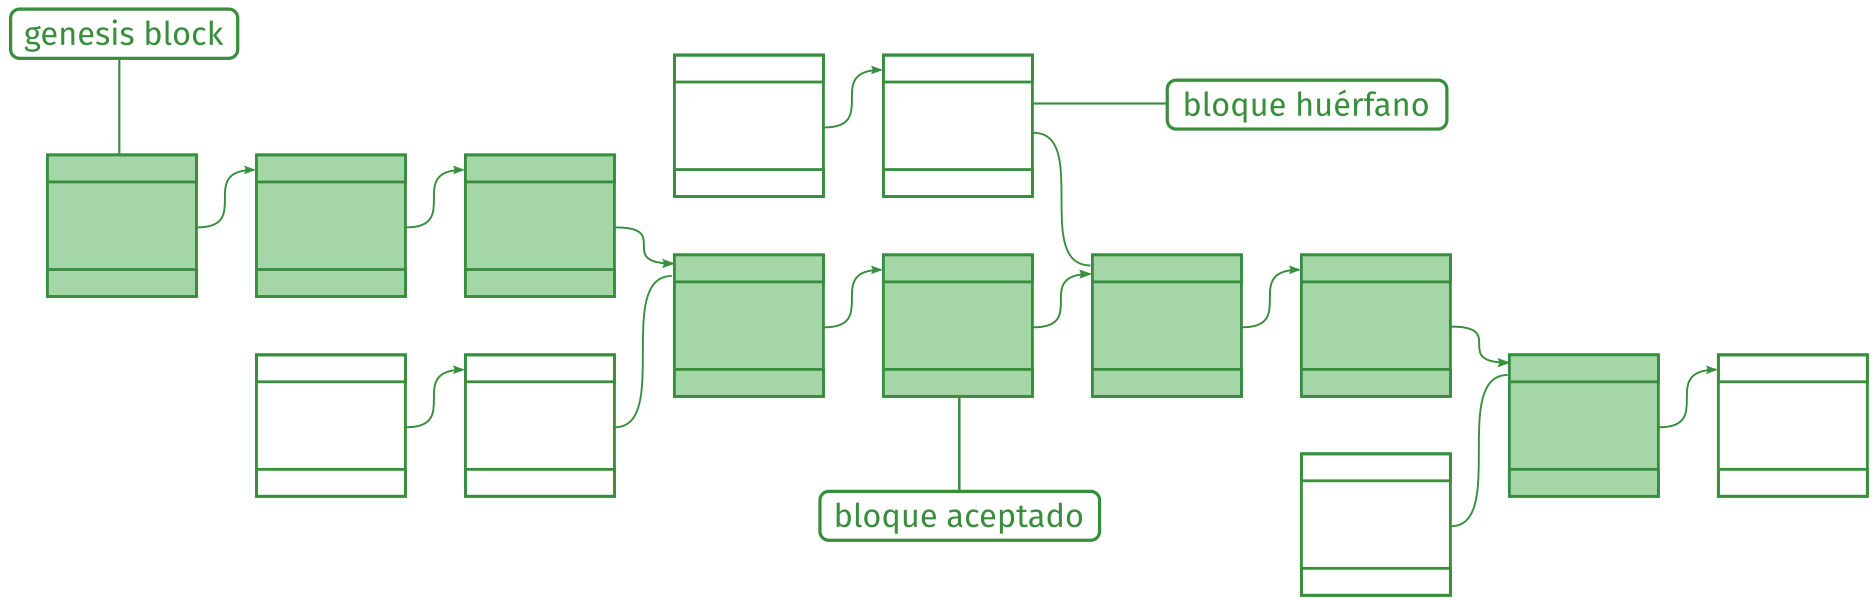
\includegraphics[width=\textwidth]{./resources/chain.png}
\end{center}	
\end{frame}

\begin{frame}{5. Mecanismos de verificación de transacciones}
Tenemos mecanismos para generar y guardar transacciones de forma descentralizada, nos
falta el factor de la confianza: \textbf{¿cómo sabemos que una transacción es cierta?}

\begin{itemize}
	\item Evitar bloques fraudulentos.
	\item El papel de los \textbf{mineros}.
\end{itemize}
\end{frame}

\begin{frame}{5. Mecanismos de verificación de transacciones. \normalfont{PoW}}
\begin{center}
	\large{\textbf{Proof-of-work}}
\end{center}
\begin{itemize}
	\item Premia a aquellos que realizan más trabajo de cómputo.
	\item Usado en Bitcoin: el minero premiado es el que consiga que el hash del bloque comience en el mayor número de ceros.
\end{itemize}
\end{frame}

\begin{frame}{5. Mecanismos de verificación de transacciones. \normalfont{PoB}}
\begin{center}
	\large{\textbf{Proof-of-burn}}
\end{center}
\begin{itemize}
	\item Criptomonedas se queman intencionadamente como una forma de ``invertir'' los recursos en la blockchain.
	\item El proceso de quema reduce la disponibilidad del mercado y aumenta el valor de la criptomoneda.
	\item Cuantas más monedas quema un usuario en favor del sistema, más poder de minería tiene.
\end{itemize}
\end{frame}

\begin{frame}{5. Mecanismos de verificación de transacciones. \normalfont{PoS}}
\begin{center}
	\large{\textbf{Proof-of-stake}}
\end{center}
\begin{itemize}
	\item Sistema centrado en propiedad de la moneda: más poder quien tenga en su cuenta más criptomonedas durante más tiempo.
	\item Un usuario compromete las criptomonedas como prueba de participación.
\end{itemize}
\end{frame}

\begin{frame}{5. Mecanismos de verificación de transacciones. \normalfont{PoET}}
\begin{center}
	\large{\textbf{Proof-of-elapsed time}}
\end{center}
\begin{itemize}
	\item Distribuir las posibilidades de ganar de manera justa entre el mayor número de participantes en la red.
\end{itemize}
\end{frame}

\begin{frame}{5. Mecanismos de verificación de transacciones. \normalfont{PoET}}
\textbf{Algoritmo PoET}
\begin{enumerate}
\item Se requiere que cada nodo participante en la red espere un período de tiempo elegido al azar, y el primero en completar el tiempo de espera designado gana el nuevo bloque.
\item
  Cada nodo en la red blockchain genera un tiempo de espera aleatorio y se va a dormir durante esa duración especificada.
\item
	El nodo que tiene el menor tiempo de espera, se despierta y envía un nuevo bloque a la cadena de bloques, transmitiendo la información necesaria a toda la red de pares.
\item
  El mismo proceso se repite para el descubrimiento del siguiente bloque.
\end{enumerate}
\end{frame}

\begin{frame}{5. Mecanismos de verificación de transacciones. \normalfont{PoI}}
\begin{center}
	\large{\textbf{Proof-of-importance}}
\end{center}
\begin{itemize}
	\item Da prioridad a los mineros con mayor \textbf{reputación} en el sistema.
	\item La reputación se mide por:
	\begin{itemize}
		\item Cantidad de dinero invertido.
		\item Número de transacciones realizadas.
		\item Cantidad transferida en dichas transacciones.
\end{itemize}
\end{itemize}
\end{frame}

\begin{frame}{6. Controlando la fuente de dinero}
\begin{center}
	\huge{¿De dónde viene el dinero?}
\end{center}	
\end{frame}


\begin{frame}{6. Controlando la fuente de dinero}
En el caso de Bitcoin, hay un límite superior de \textbf{21M BTC}, y el dinero incrementa con las \textbf{recompensas de los mineros}.

Esta recompensa se calcula a partir de tres factores:
\begin{itemize}
	\item Dinero que hay en el sistema.
	\item Trabajo computacional de los mineros.
	\item Dificultad del mineo.
\end{itemize}

Además, hemos de incluir en el juego las \textbf{tarifas de transacción}.
\end{frame}

\section{Demo: Bitcoin Core}

\begin{frame}{Procedimiento seguido}
\begin{enumerate}
	\item Descargamos \textbf{Bitcoin Core} de la página web oficial.
	\item Iniciamos \textbf{Wireshark}.
	\item Ejecutamos el cliente \texttt{bitcoin-qt}.
	\begin{itemize}
		\item Se descargarán todos los bloques de Bitcoin en \texttt{\textasciitilde/.bitcoin}.
		\item ¡Más de 200GB!
\end{itemize}
\end{enumerate}
\end{frame}

\begin{frame}{Procedimiento seguido}
\begin{center}
	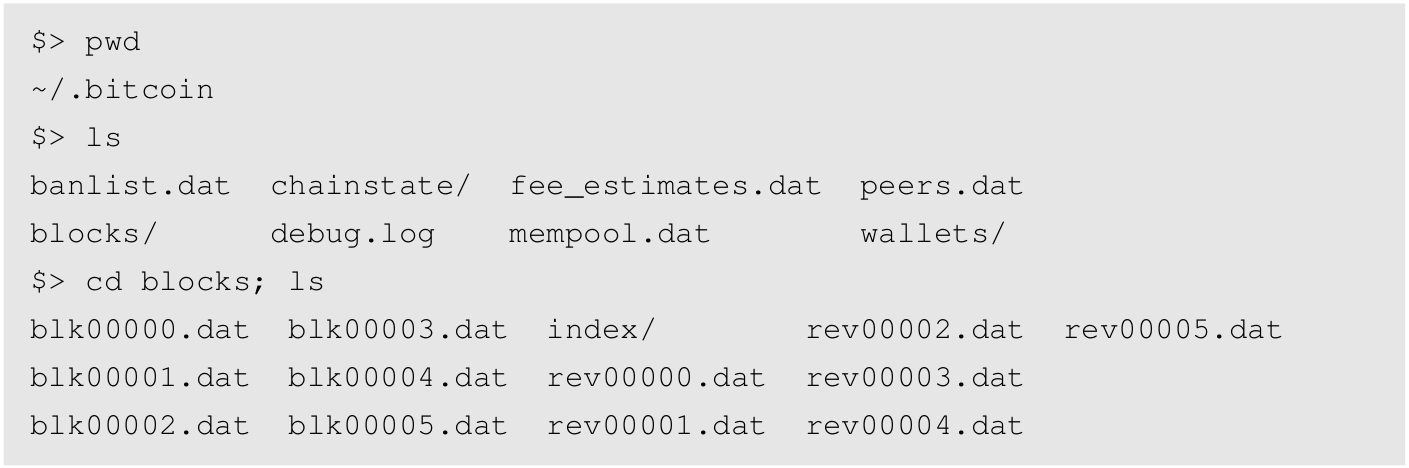
\includegraphics[width=\textwidth]{./resources/scr1.png}
\end{center}	
\end{frame}

\begin{frame}{Formato del bloque}
\begin{center}
	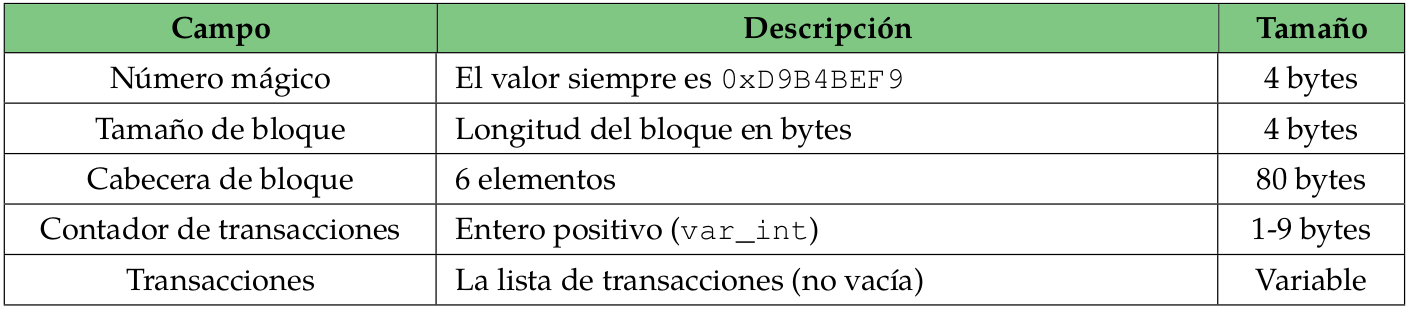
\includegraphics[width=\textwidth]{./resources/scr2.png}
\end{center}	
\end{frame}

\begin{frame}{Formato del bloque. \normalfont{Número mágico}}
\begin{center}
Siempre es \texttt{0xD9B4BEF9}\\
\hspace{1cm}
	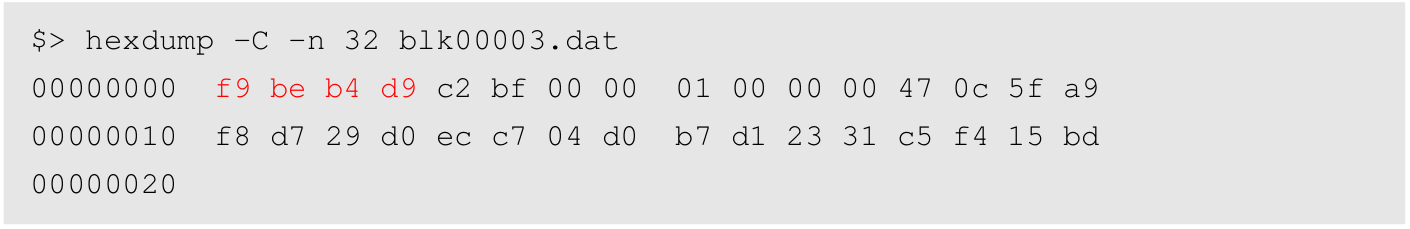
\includegraphics[width=\textwidth]{./resources/scr3.png}
\end{center}	
\end{frame}

\begin{frame}{Formato del bloque. \normalfont{Tamaño de bloque}}
\begin{center}
\texttt{0x0000BFC2} $\longrightarrow$ 49090 bytes\\
\hspace{1cm}
	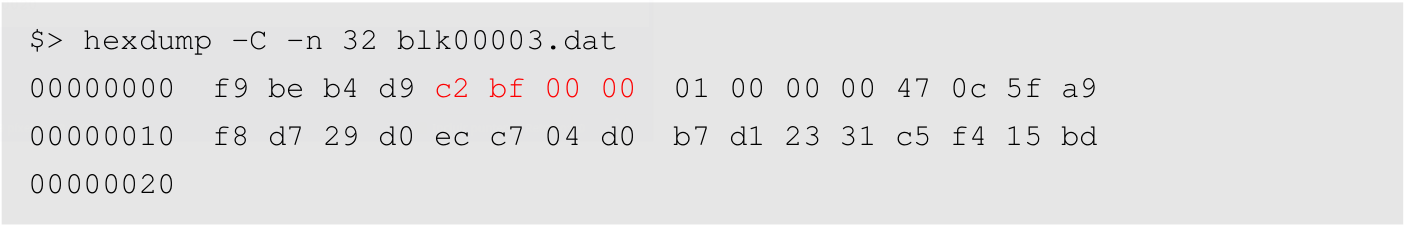
\includegraphics[width=\textwidth]{./resources/scr4.png}
\end{center}	
\end{frame}

\begin{frame}{Formato del bloque. \normalfont{Cabecera del bloque}}
\begin{center}
\hspace{1cm}
	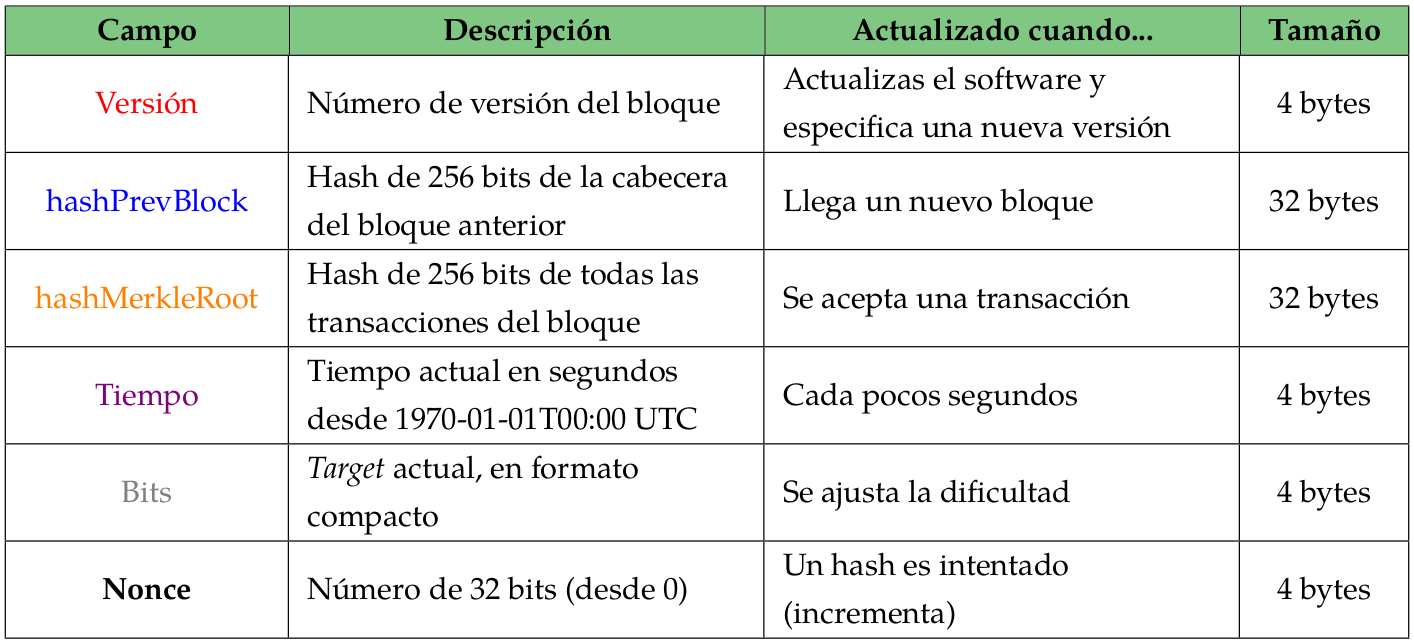
\includegraphics[width=\textwidth]{./resources/scr5.png}
\end{center}	
\end{frame}

\begin{frame}{Formato del bloque. \normalfont{Cabecera del bloque}}
\begin{center}
\hspace{1cm}
	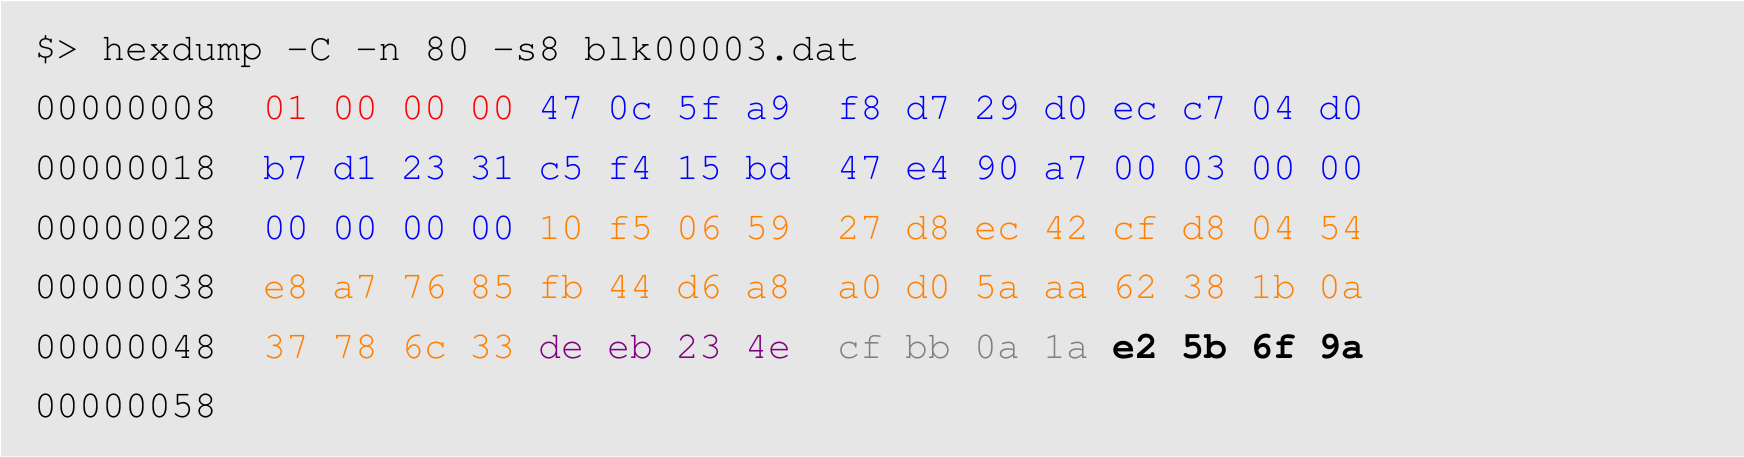
\includegraphics[width=\textwidth]{./resources/scr6.png}
\end{center}	
\end{frame}

\begin{frame}{Formato del bloque. \normalfont{Cabecera del bloque}}
\begin{itemize}
\item
  \textbf{Versión:} \texttt{0x00000001}.
\item
  \textbf{hashPrevBlock:} \texttt{0x0000000000000300A790E447BD}...
\item
	\textbf{hashMerkleRoot:} \texttt{0x336C78370A1B3862AA5AD0A0A8}...
\item
	\textbf{Tiempo:} \texttt{0x4E23EBDE} $\longrightarrow$ 1310976990 \\$\longrightarrow$ 18 de julio de 2011, a las 08:16:30 UTC.
\item
	\textbf{Bits:} \texttt{0x1A0ABBCF}, codificación de punto flotante.
\begin{itemize}
	\item
		El exponente es \texttt{0x1A} = 26.
	\item
		La mantisa es \texttt{0x0ABBCF}.
	\item
		Exponente dice que este es un entero de 26 bytes y base 256. Le añadimos 23 ceros hasta obtener: \texttt{0a bb cf 00 00   00 00 00 00 00    00 00 00 00 00    00 00 00 00 00    00 00 00 00    00 00}.
	\item
		Este número, convertido a decimal, es:$$0x0a * 256^{26} + 0xbb * 256^{25} + 0xcf*256^{24} \approx  4.4155582e63$$
	\end{itemize}
\item
	\textbf{Nonce}: \texttt{0x9A6F5BE2}.	
\end{itemize}
\end{frame}

\begin{frame}{Formato del bloque. \normalfont{Contador de transacciones}}
\begin{center}
\hspace{1cm}
	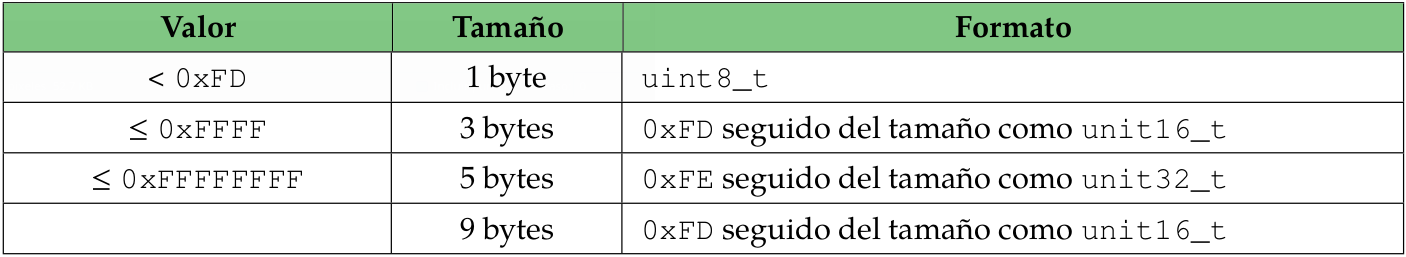
\includegraphics[width=\textwidth]{./resources/scr7.png}
\end{center}	
\end{frame}

\begin{frame}{Formato del bloque. \normalfont{Contador de transacciones}}
\begin{center}
\texttt{0x9A} $\longrightarrow$ 154 transacciones\\
\hspace{1cm}
	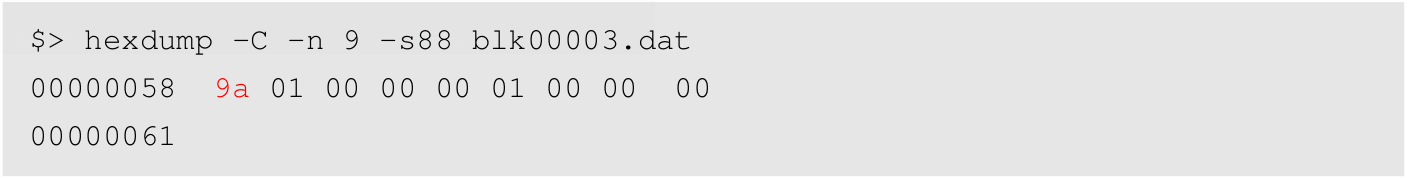
\includegraphics[width=\textwidth]{./resources/scr8.png}
\end{center}	
\end{frame}

\begin{frame}{Formato del bloque. \normalfont{Transacciones}}
\begin{center}
Primera transacción del bloque: \textbf{recompensa del minero}\\
\hspace{1cm}
	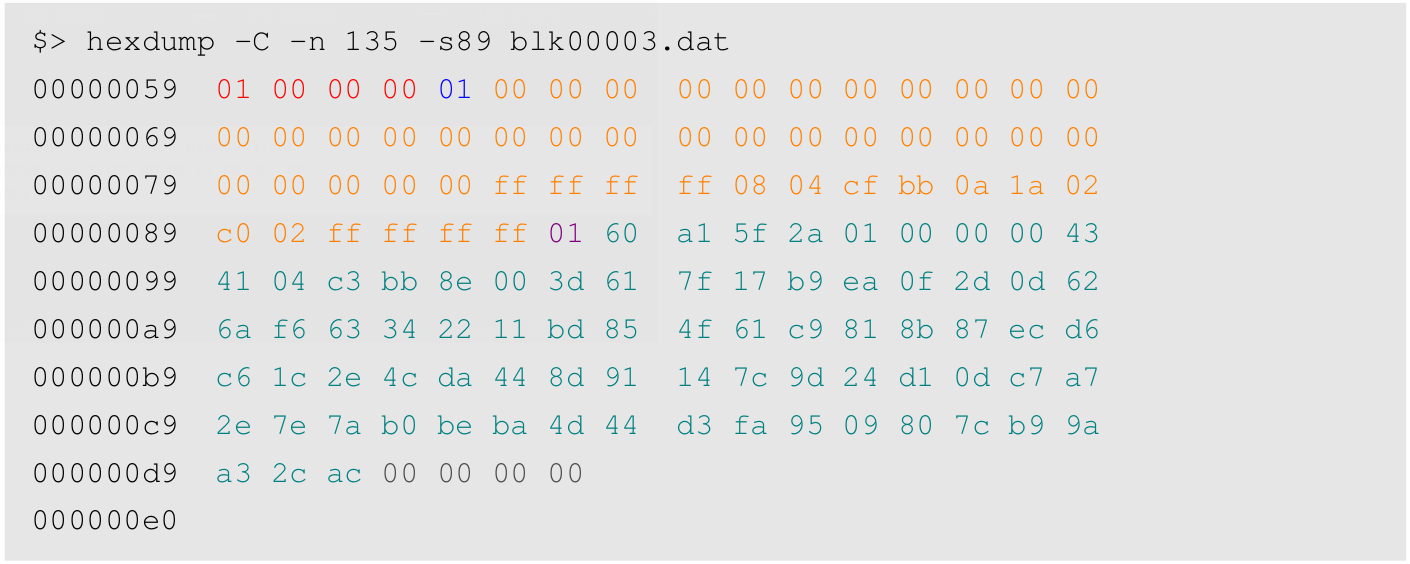
\includegraphics[width=\textwidth]{./resources/scr9.png}
\end{center}	
\end{frame}

\begin{frame}{Formato del bloque. \normalfont{Transacciones}}
\begin{center}
	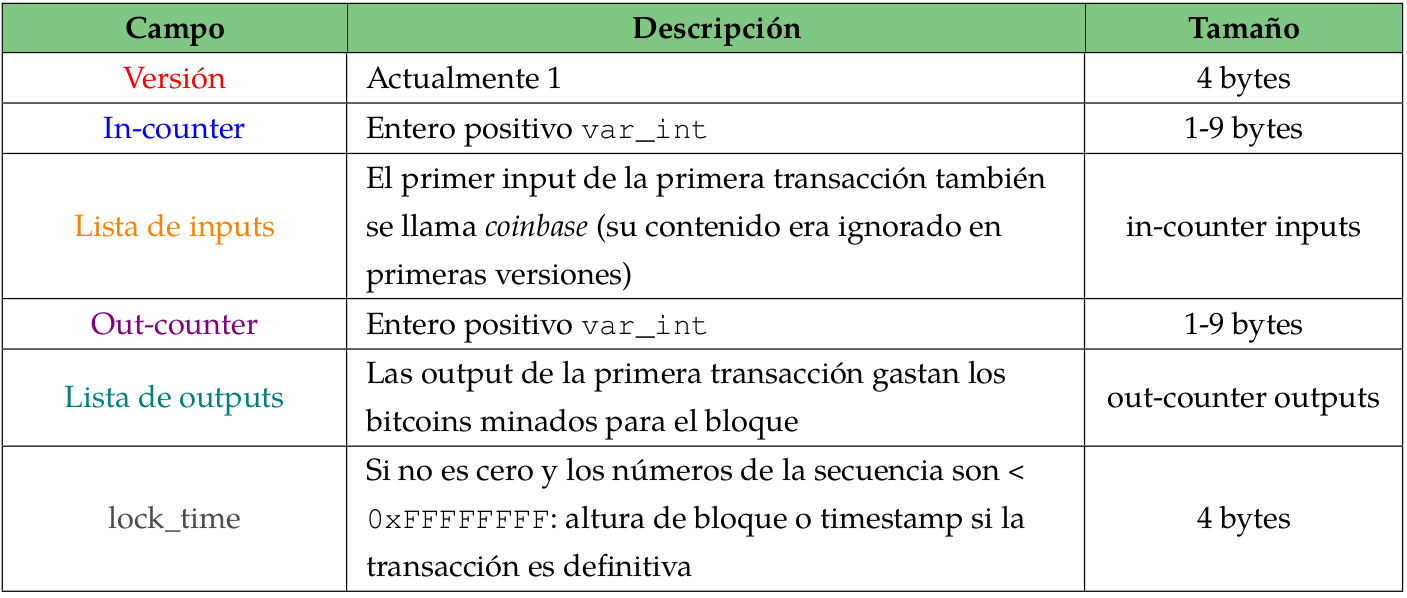
\includegraphics[width=\textwidth]{./resources/scr10.png}
\end{center}	
\end{frame}

\begin{frame}{Formato del bloque. \normalfont{Transacciones}}
\begin{center}
\vspace{0.5cm}
	\huge{50 BTC}\large{, julio 2011}
	
	\huge{$\downarrow$}
	
	\vspace{0.3cm}
	
	\huge{12.5 BTC}\large{, hoy}

	\vspace{0.3cm}	
	
	\hspace{0.2cm}\large{\color{white}{\emph{halving}}}\huge{$\downarrow$}\hspace{0.2cm}\large{\emph{halving}}
	
	\vspace{0.3cm}
	
	\huge{6.25 BTC}\\\large{23 mayo 2020 06:29:48}
\end{center}	
\end{frame}

\begin{frame}{Formato del bloque. \normalfont{Transacciones}}
\begin{center}
\Large{\textbf{Input}}\\
\hspace{1cm}
	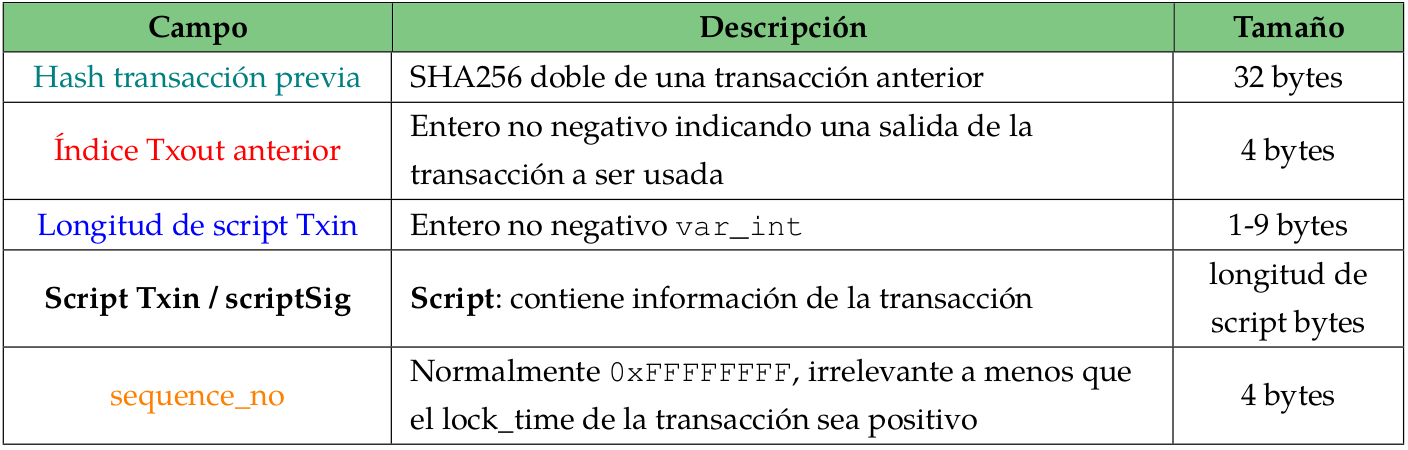
\includegraphics[width=\textwidth]{./resources/scr11.png}
\end{center}	
\end{frame}

\begin{frame}{Formato del bloque. \normalfont{Transacciones}}
\begin{center}
Transacción \emph{coinbase}\\
\hspace{1cm}
	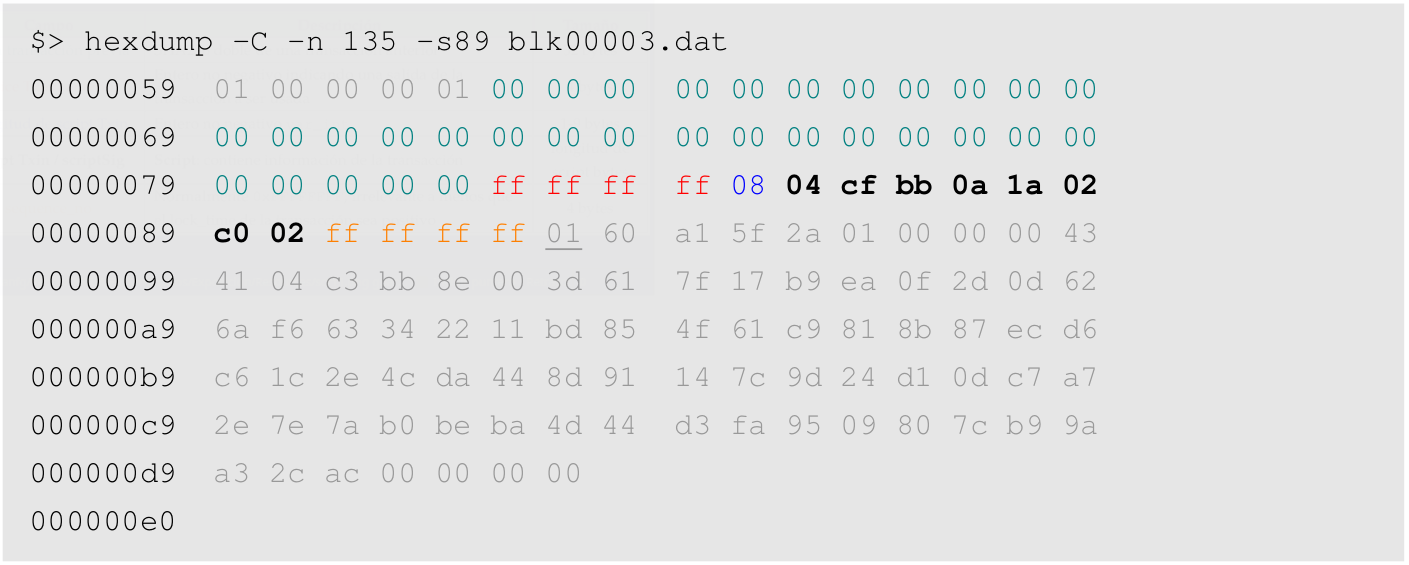
\includegraphics[width=\textwidth]{./resources/scr12.png}
\end{center}	
\end{frame}

\begin{frame}{Formato del bloque. \normalfont{Transacciones}}
\begin{center}
\Large{\textbf{Output}}\\
\hspace{1cm}
	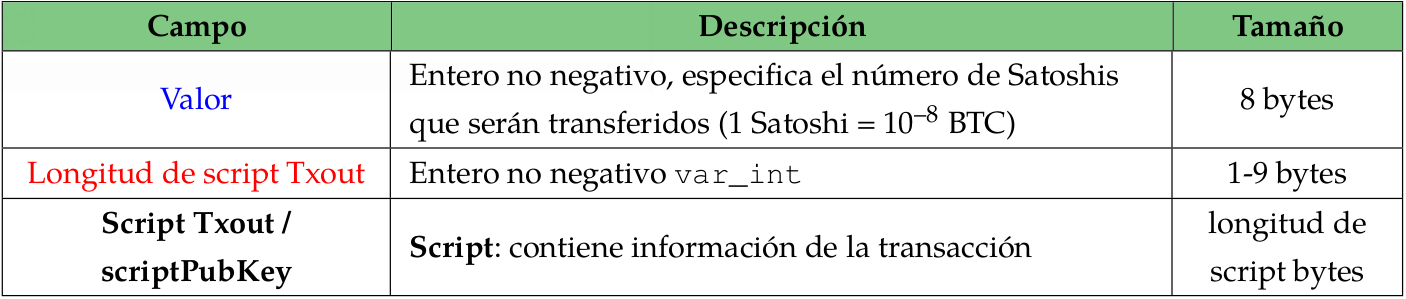
\includegraphics[width=\textwidth]{./resources/scr13.png}
\end{center}	
\end{frame}

\begin{frame}{Formato del bloque. \normalfont{Transacciones}}
\begin{center}
\texttt{0x000000012A5FA160} $\longrightarrow$ 5005877600 Satoshis $\longrightarrow$ 50.058776 BTC \\
\hspace{1cm}
	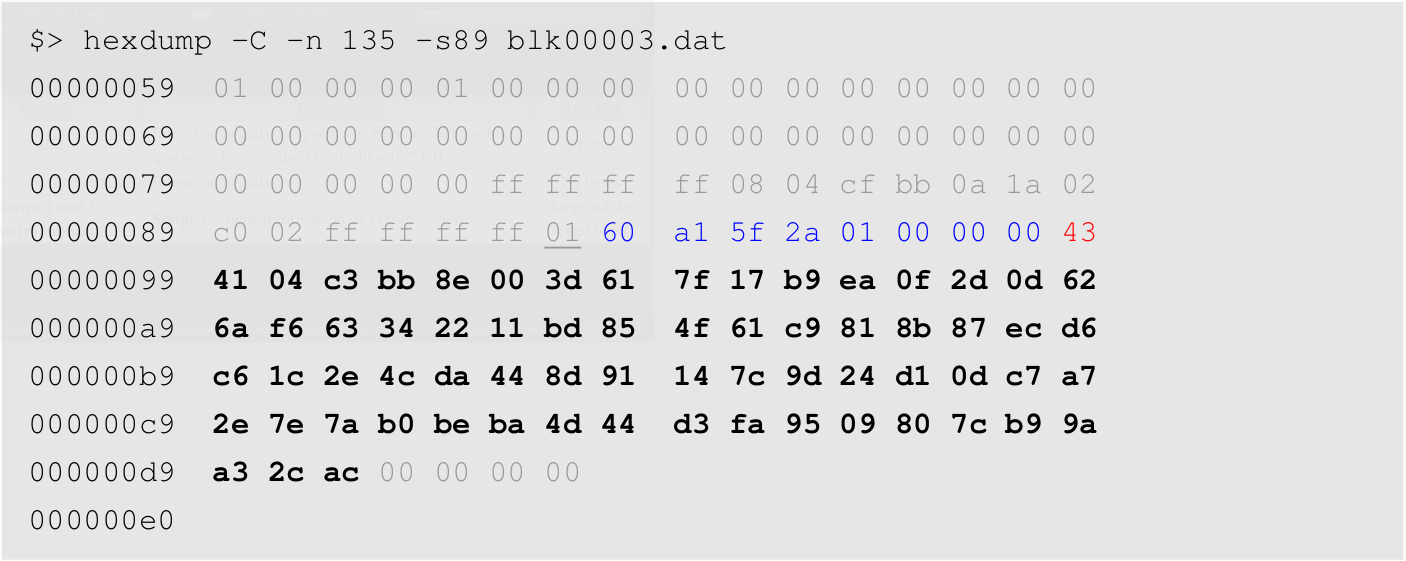
\includegraphics[width=\textwidth]{./resources/scr14.png}
\end{center}	
\end{frame}

\begin{frame}{Análisis de mensajes}
\vspace{-0.3cm}
\begin{center}
	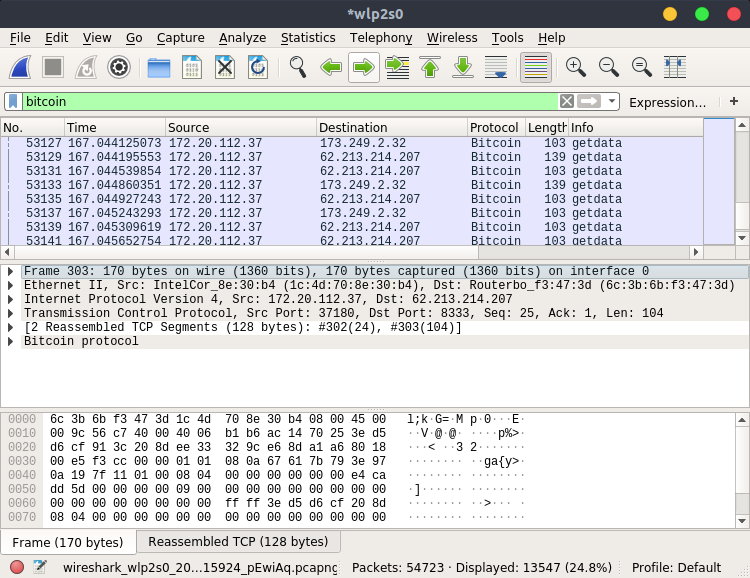
\includegraphics[width=\textwidth]{./resources/wireshark0.png}
\end{center}	
\end{frame}

\begin{frame}{Análisis de mensajes. \normalfont{Estructura general}}
\begin{center}
Nodos Bitcoin se conectan entre sí por TCP,\\buscando normalmente en el puerto 8333 \\
\hspace{1cm}
	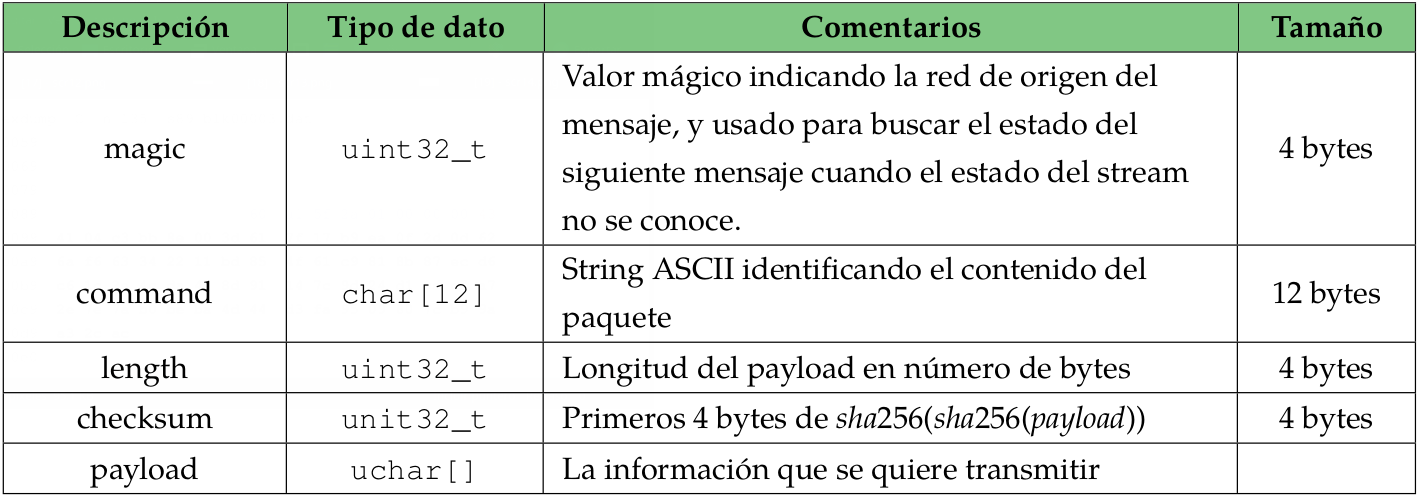
\includegraphics[width=\textwidth]{./resources/scr15.png}
\end{center}	
\end{frame}

\begin{frame}{Análisis de mensajes. \normalfont{Estructura general}}
\begin{center}
Número mágico, en \emph{little endian} \\
\hspace{1cm}
	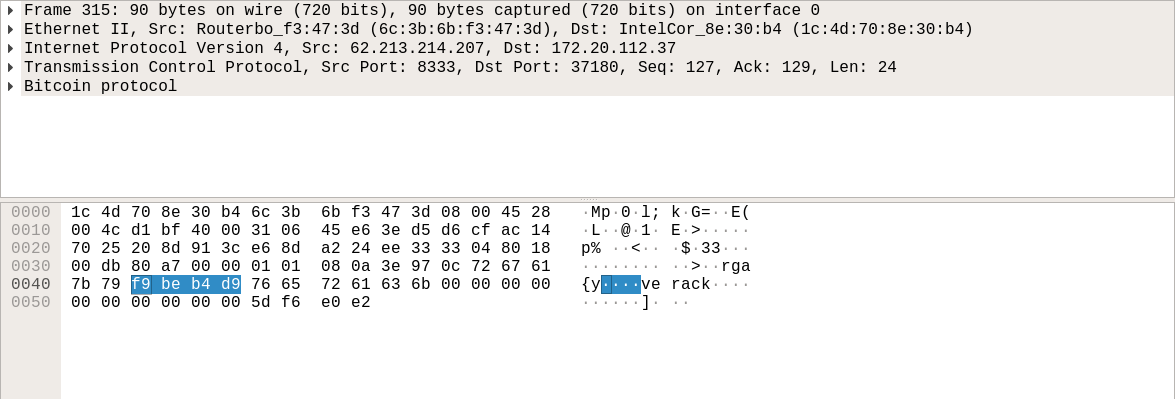
\includegraphics[width=\textwidth]{./resources/wireshark1.png}
\end{center}	
\end{frame}

\begin{frame}{Análisis de mensajes. \normalfont{Estructura general}}
\begin{center}
Mensaje \texttt{verack}, en respuesta a \texttt{version} \\
\hspace{1cm}
	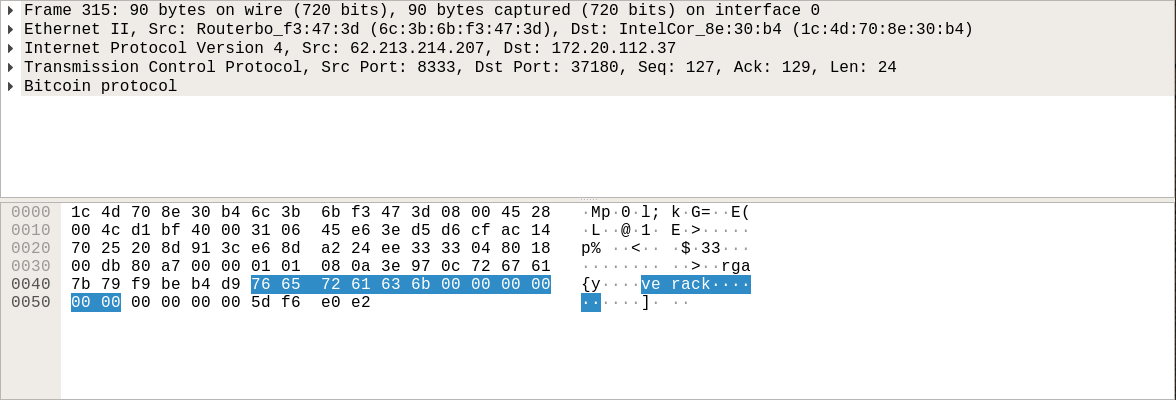
\includegraphics[width=\textwidth]{./resources/wireshark2.png}
\end{center}	
\end{frame}

\begin{frame}{Análisis de mensajes. \normalfont{Analizando un mensaje: \texttt{block}}}
\begin{center}
Mensaje \texttt{block}, en respuesta a \texttt{getdata} \\
\hspace{1cm}
	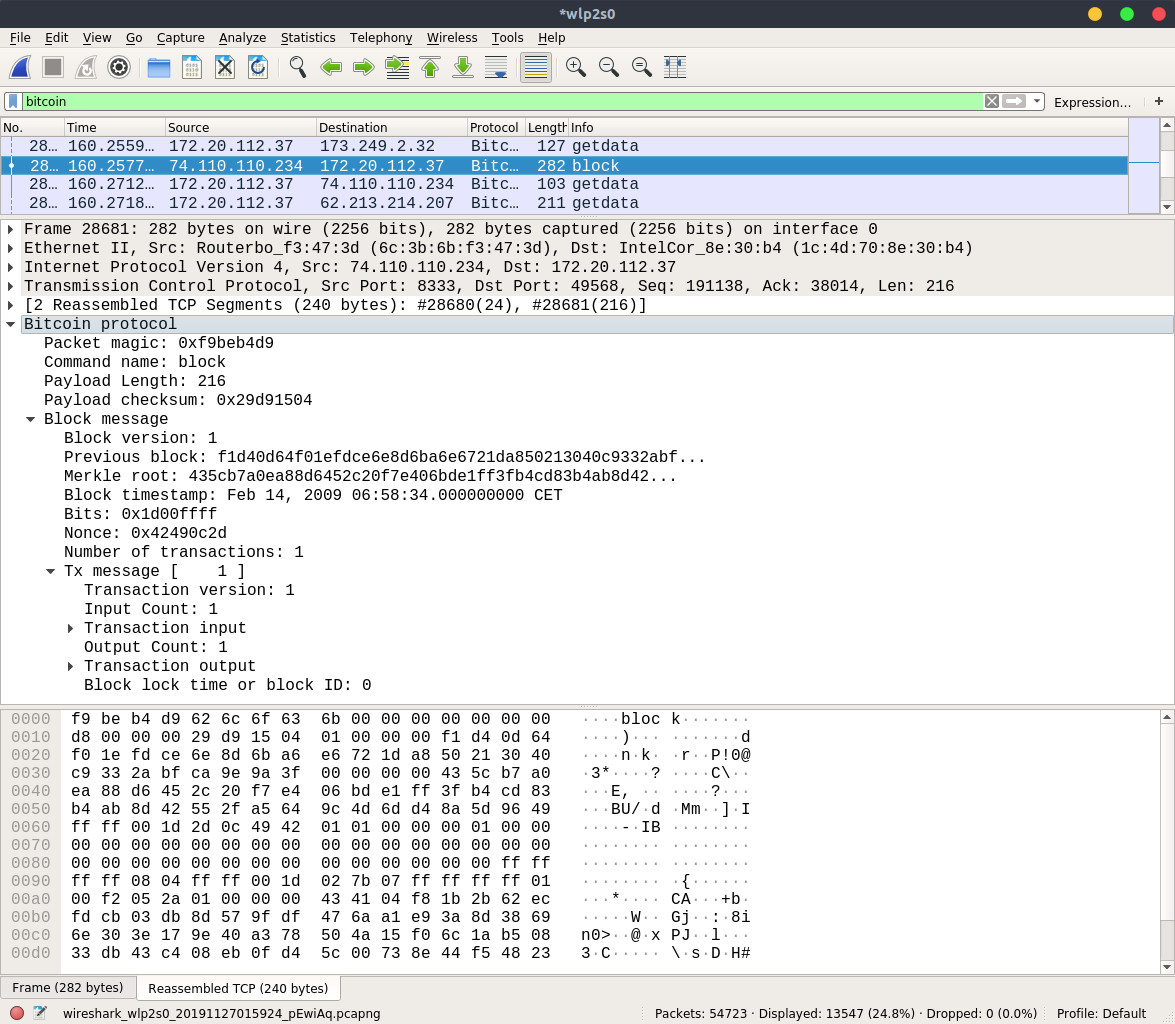
\includegraphics[width=\textwidth]{./resources/wireshark3.png}
\end{center}	
\end{frame}

\begin{frame}{Análisis de mensajes. \normalfont{Analizando un mensaje: \texttt{block}}}
\begin{center}
	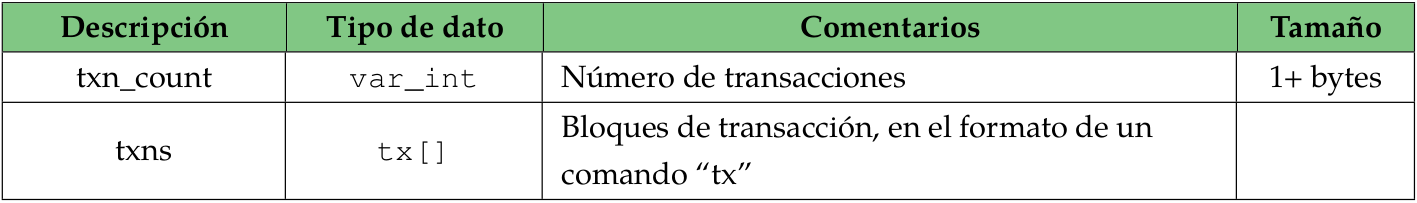
\includegraphics[width=\textwidth]{./resources/scr16.png}
\end{center}	
\end{frame}

\begin{frame}{Análisis de mensajes. \normalfont{Analizando un mensaje: \texttt{block}}}
\begin{center}
5000000000 Satoshis $\longrightarrow$ 50 BTC \\
\hspace{1cm}
	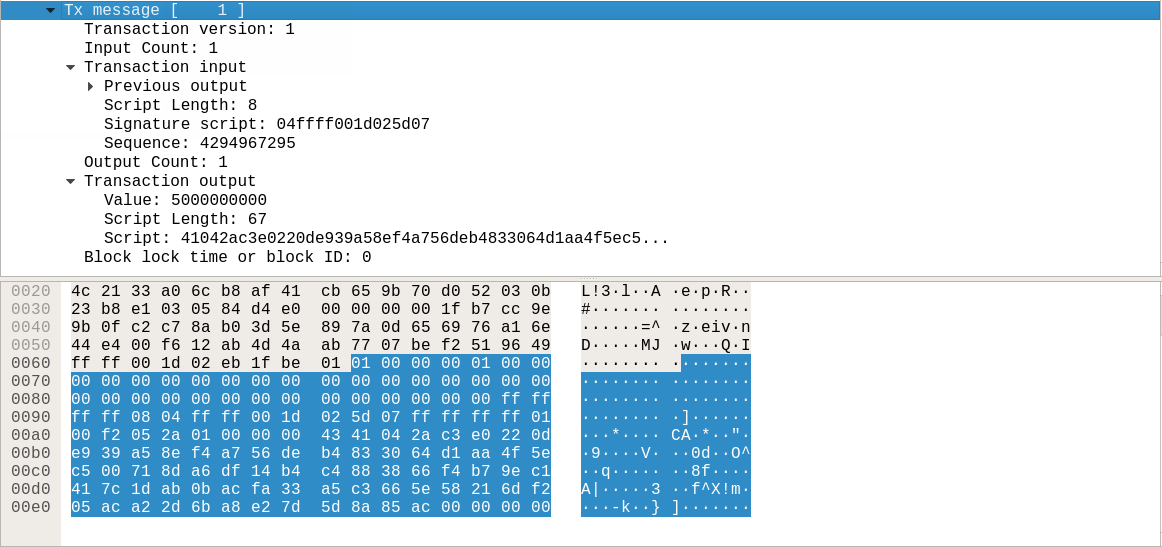
\includegraphics[width=\textwidth]{./resources/wireshark4.png}
\end{center}
\end{frame}

\begin{frame}[standout]
	¡Gracias por vuestra atención!
\end{frame}
\end{document}
